% !TeX spellcheck = en_US
\documentclass[french]{yLectureNote}

\title{Optique ondulatoire}
\subtitle{Physique}
\author{Paulhenry Saux}
\date{\today}
\yLanguage{Français}

\professor{F.Pettinari}
\usepackage{graphicx}%----pour mettre des images
\usepackage[utf8]{inputenc}%---encodage
\usepackage{geometry}%---pour modifier les tailles et mettre a4paper
%\usepackage{awesomebox}%---pour les boites d'exercices, de pbq et de croquis ---d\'esactiv\'e pour les TP de PC
\usepackage{tikz}%---pour deiffner + d\'ependance de chemfig
% \usepackage{tabularx}%---pour dimensionner automatiquement les tableaux avec variable X
\usepackage{awesomebox}%---Pour les boites info, danger et autres
\usepackage{menukeys}%---Pour deiffner les touches de Calculatrice
\usepackage{fancyhdr}%---pour les en-t\^ete personnalis\'ees
\usepackage{blindtext}%---pour les liens
\usepackage{hyperref}%---pour les liens (\`a mettre en dernier)
\usepackage{caption}%---pour la francisation de la l\'egende table vers Tableau
\usepackage{pifont}
\usepackage{array}%---pour les tableaux
\usepackage{lipsum}
\usepackage{yFlatTable}
\usepackage{multicol}
\newcommand{\Lim}[1]{\lim\limits_{\substack{#1}}\:}
\renewcommand{\vec}{\overrightarrow}
\newcommand{\N}[0]{\mathbb{N}}
\newcommand{\dd}{\mathrm{d}}
\newcommand{\norm}[1]{||\vec{#1}||}
\newcommand{\fo}{\psi(\vec{r},t)}
\newcommand{\foe}{\psi(\vec{r},t)\*}
\newcommand{\HH}{\hat{H}}
\newcommand{\hb}{\hbar}
\newcommand{\lap}{\nabla^2}
\newcommand{\lapcc}{\frac{\partial^2 }{\partial x^2}+\frac{\partial^2 }{\partial y^2}+\frac{\partial^2 }{\partial z^2}}
\newcommand{\mpsi}{\(\psi\)}
\newcommand{\und}{\underline}
\newcommand{\dph}{\Delta\varphi}
\begin{document}
\chapter{TP électro-magnétisme}
\section{Mesure de e/m}
\subsection{Fonctionnement du canon à électron}
\begin{enumerate}
 \item L'émission thermoïonique : Tout commence par un filament  chauffé par un courant électrique. Sous l'effet de la chaleur, les électrons du métal reçoivent assez d'énergie pour s'en échapper : c'est l'effet thermoïonique.

\item La focalisation (Le cylindre de Wehnelt) : Une électrode cylindrique entourant la cathode, chargée négativement, repousse les électrons vers l'axe central pour commencer à former un faisceau fin.

\item L'accélération : Une anode (électrode positive) placée plus loin crée un champ électrique intense. Puisque les électrons sont chargés négativement, ils sont violemment attirés par cette anode, ce qui leur confère une grande vitesse cinétique.

\item Le guidage : Une fois lancés, les électrons passent par un petit orifice dans l'anode pour former un pinceau lumineux qui sera ensuite dirigé vers sa cible.
\end{enumerate}
\subsection{À savoir : Protocole avec R constant}
\subsubsection{Mesures}
\begin{enumerate}
 \item Placer la tension du générateur à 130V environ
 \item Placer le premier marqueur de mesure à l'origine du faisceau
 \item Régler l'intensité des bobines pour observer un diamètre de 11.6cm environ
 \item Relever la paire Tension/Intensité
 \item Augmenter la tension du générateur jusqu'à 300V par pas de 20V et refaire les étapes 2 et 3
\end{enumerate}
\subsubsection{Modélisation}
\begin{itemize}
 \item $B^2 = f(U) = A\cdot U$
 \item Valeur théorique (utile pour comparer les résultats) : $1,75882 \cdot 10^{11} SI$.
\end{itemize}

\subsection{À savoir : Protocole avec tension constante}
\subsubsection{Mesures}
\begin{enumerate}
 \item Placer la tension du générateur à 200V environ
  \item Placer le premier marqueur de mesure à l'origine du faisceau
 \item Régler l'intensité des bobines à 1A
 \item Relever le diamètre du cercle de la trajectoire adoptée par les électrons
 \item Pour des valeurs de I de 1 à 2.1A par pas de 0.1, refaire l'étape précédente.
\end{enumerate}
\subsubsection{Modélisation}
\begin{enumerate}
 \item $r^2 = f(B^{-2}) = C\cdot B^{-2}$
\end{enumerate}
\section{Magnétisme}
\begin{itemize}
 \item Lors des modélisations en fonction de x, il faut utiliser plutot \(x-x_0\) en raison de l'imprecision de la sonde.
 \item Penser à étalloner la sonde entre chaque série de mesure !
 \item Sur certains multimètre, il faut appuyer sur DCI pour activer l'ampère-mètre et DCV pour le voltmètre.
\end{itemize}
\section{Résonnance}
\subsection{Résonnance en intensité}
\subsubsection{Montage expérimental}
Nous réalisons le montage indiqué en figure 1. Par convention, on associe la mesure de la tension du générateur au canal 1 et celle de la résistance au canal 2.
\begin{center}
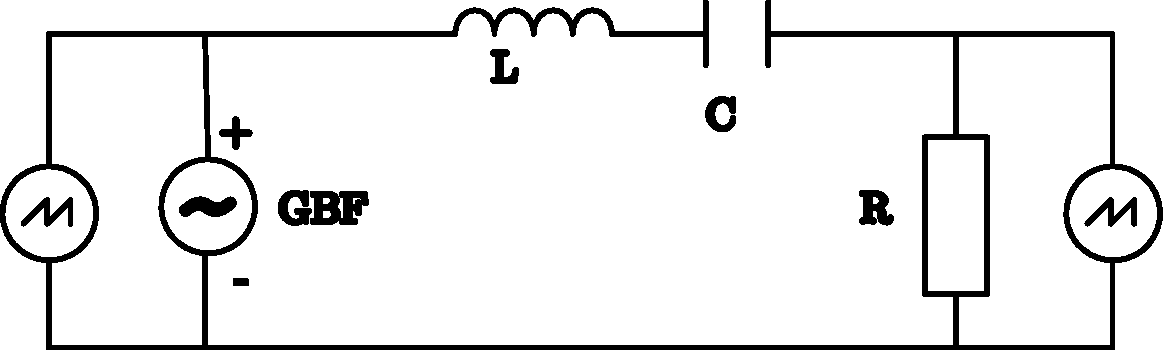
\includegraphics[scale=0.3]{circuit1}
\end{center}
\subsubsection{À savoir}
\begin{itemize}
 \item $Q = \frac{1}{R}\sqrt{\frac{L}{C}}$
 \item Pour le déphasage, relever la valeur CH2-CH1 (en bleue) et non celle de CH1-CH2
 \item On peut modifier la finnesse du bouton de modification de l'échelle verticale de l'oscilloscope avec le boutton ``function''
 \item La bobine L possède une résistance interne r. Dans les calculs de Q, la "vraie" résistance \(R_t\)​ est \(R​+r\).
\end{itemize}

\subsection{Résonnance en charge}
\subsubsection{Description du montage expérimental}
Nous réalisons le montage indiqué en figure 2. Par convention, on associe la mesure de la tension du générateur au canal 1 et celle de la résistance au canal 2.
\begin{center}
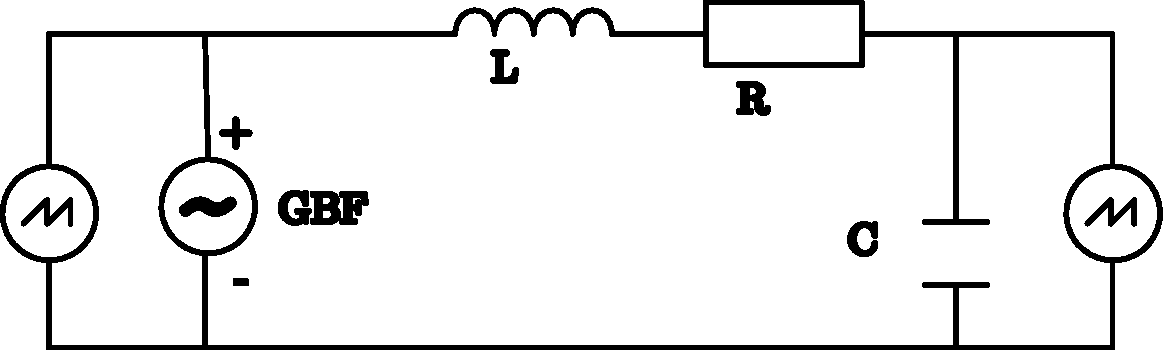
\includegraphics[scale=0.3]{circuit2}
\end{center}
\subsubsection{À savoir}
\begin{itemize}
 \item $Q = \frac{\sqrt{LC}}{RC}$
\end{itemize}

 \end{document}
